\setcounter{section}{4}
\section{TP05 - Regular expressions}
{
\renewcommand{\thesubsubsection}{\thesubsection\alph{subsubsection}}
\subsection{Exercise 1}
\subsubsection{Item a}
\begin{alignat*}{3}
	(\varepsilon + a + aa + aaa)(baaa)^*(\varepsilon + b + ba + baa)
\end{alignat*}
\subsubsection{Item b}
I prefer an $\varepsilon$-NFA because it simplifies the task of recognizing the $\varepsilon$'s of the regular expression when converting from RE to a FA.
\subsubsection{Item c}
\begin{center} \includegraphics[scale=0.5]{TP05_1_c_0} \end{center}
This $\varepsilon$-NFA can be trivially converted to the following incomplete DFA.
\begin{center} \includegraphics[scale=0.5]{TP05_1_c_1} \end{center}
\subsection{Exercise 2}
\subsubsection{Item a}
\begin{alignat*}{3}
	 (aa)^* (b  (aa)^* ( b + aba ) + ab (aa)^* ( ab + ba ))(aa)^*
\end{alignat*}
\subsubsection{Item b}
Yes it can. Convert the RE to an $\varepsilon$-NFA and then to a DFA $D$. Then, create the DFA $\overline{D}$ describing the complement of $D$ by converting accept states to normal states, and normal states to accept states. Then, convert $\overline{D}$ to a RE.
\pagebreak
\subsection{Exercise 3}
\begin{equation*}
	(0 + 10)^* 11 (0 + 01)^*
\end{equation*}
\subsection{Exercise 4}
\subsubsection{Item a}
Strings with a maximum of one subsequence of consecutive $1$'s, which can only happen at the end.
\subsubsection{Item b}
Strings with at least one subsequence of three consecutive $0$'s.
\subsubsection{Item c}
Strings with no consecutive $1$'s.
\subsection{Exercise 5}
\begin{center} \begin{tabular}{r | l}
	\textbf{Item} & \textbf{Answer} \\ \hline
	a & False \\
	b & True \\
	c & True \\
	d & True
\end{tabular} \end{center}
\subsubsection{Item a}
False, given the string $a$ is accepted by $(a+b)^*$ but not by $(a^* b)^*$.
\subsubsection{Item b}
True, given it can be converted into a DFA, and then into a RE.
\subsubsection{Item c}
True, given $S^*$ is defined by $S \subseteq S^*$ and $v,w \in S^* \implies v+w \in S^*$ means the concatenation of any two strings of $S^*$ was already in $S^*$.
\subsubsection{Item d}
True. The proof is the fact there is an algorithm that transforms a regular expression describing a language with concatenation, union and closure into an $\varepsilon$-DFA, and another algorithm to transform the $\varepsilon$-DFA into a DFA.
\subsection{Exercise 6}
\subsubsection{Item a}
\begin{center}
\begin{tabular}{c c}
\includegraphics[scale=0.5]{TP05_6_a_1} &
\includegraphics[scale=0.5,trim={0 22mm 0 0}]{TP05_6_a_2} \\
\includegraphics[scale=0.5,trim={0 22mm 0 0}]{TP05_6_a_3} &
\includegraphics[scale=0.5,trim={0 21mm 0 0}]{TP05_6_a_4}
\end{tabular}
\end{center}
\begin{equation*}
	\text{a}(\oplus (\text{c} \otimes )^* \text{b})^* .
\end{equation*}
\subsubsection{Item b}
\begin{equation*}
	\text{a}.
\end{equation*}
\subsubsection{Item c}
An infinite number of strings, given the use of the closure operator $^*$.
\pagebreak
\subsection{Exercise 7}
\subsubsection{Item a}
\begin{center}
\begin{minipage}{0.35\textwidth}
\begin{center} \begin{tabular}{r | c c c}
	$\delta_E     $ & $\varepsilon$ & $0        $ & $1        $ \\ \hline
	$\rightarrow A$ & $\{C      \}$ & $\{B    \}$ & $\emptyset$ \\
	$            B$ & $\emptyset  $ & $\emptyset$ & $\{D    \}$ \\
	$            C$ & $\emptyset  $ & $\{C    \}$ & $\{C,D  \}$\\
	$      ^* D$ & $\emptyset  $ & $\emptyset$ & $\emptyset$
\end{tabular} \end{center}
\end{minipage}%
\begin{minipage}{0.25\textwidth}
	\begin{alignat*}{2}
		\varepsilon close(A)&=\{A,C\}\\
		\varepsilon close(B)&=\{B\}\\
		\varepsilon close(C)&=\{C\}\\
		\varepsilon close(D)&=\{D\}\\
	\end{alignat*}
\end{minipage}
\end{center}
\begin{center}
\begin{minipage}[c]{0.44\textwidth}
	\begin{alignat*}{2}
		DFA\,D    &= (Q_D, \Sigma, \delta_D, q_0, F_D)\\
		Q_D      &= \{\{C\},\{A,C\},\{B,C\},\{C,D\}\}\\
		\Sigma   &= \{0,1\}\\
		q_0      &= \{A,C\}\\
		F_D      &= \{\{C,D\}\}\\
		\delta_D &\colon Q_D \times \Sigma \rightarrow Q_D
	\end{alignat*}
\end{minipage}%
\begin{minipage}[c]{0.32\textwidth}
\begin{center} \begin{tabular}{r | c c}
	$\delta_D           $ & $0      $ & $1      $ \\ \hline
	$            \{C  \}$ & $\{C  \}$ & $\{C,D\}$ \\	
	$\rightarrow \{A,C\}$ & $\{B,C\}$ & $\{C,D\}$ \\
	$            \{B,C\}$ & $\{C  \}$ & $\{C,D\}$ \\
	$      ^* \{C,D\}$ & $\{C  \}$ & $\{C,D\}$
\end{tabular} \end{center}
\end{minipage}%
\begin{minipage}[c]{0.24\textwidth}
	\begin{center} \includegraphics[scale=0.5]{TP05_7_a} \end{center}
\end{minipage}
\end{center}
\subsubsection{Item b}
\begin{center} \includegraphics[scale=0.5]{TP05_7_b_1} \end{center}
\begin{center} \includegraphics[scale=0.5]{TP05_7_b_2} \end{center}
\begin{center} \includegraphics[scale=0.5]{TP05_7_b_3} \end{center}
\begin{equation*}
	01+(0+1)^* 1 = (0+(0+1)^*) 1 = (0+1)^* 1
\end{equation*}
\pagebreak
\subsection{Exercise 8}
\subsubsection{Item a}
\begin{center} \includegraphics[scale=0.5]{TP05_8_a} \end{center}
$ab$, $abab$, $aba$ are accepted.
\subsubsection{Item b}
Language of strings started in $a$ with no consecutive $b$'s and at most two consecutive $a$'s.
\subsubsection{Item c}
\begin{center} \begin{tabular}{c c c}
\includegraphics[scale=0.5]{TP05_8_c_1} &
\includegraphics[scale=0.5]{TP05_8_c_2} &
\includegraphics[scale=0.5,trim={0 7mm 0 0}]{TP05_8_c_3} 
\end{tabular} \end{center}
\begin{equation*}
	ab(\varepsilon+a)(ab(\varepsilon+a))^*=(ab(\varepsilon+a))^+
\end{equation*}
\subsubsection{Item d}
\begin{center}
\begin{minipage}{0.30\textwidth}
	\begin{center} \begin{tabular}{r | c c}
		$\delta_D           $ & $a        $ & $b        $\\ \hline
		$          \emptyset$ & $\emptyset$ & $\emptyset$\\
		$\rightarrow \{0  \}$ & $\{1    \}$ & $\emptyset$\\
		$            \{1  \}$ & $\emptyset$ & $\{2,3  \}$\\
		$      ^* \{1,3\}$ & $\{1    \}$ & $\{2,3  \}$\\
		$      ^* \{2,3\}$ & $\{1,3  \}$ & $\emptyset$
	\end{tabular} \end{center}
\end{minipage}
\begin{minipage}{0.30\textwidth}
	\begin{center} 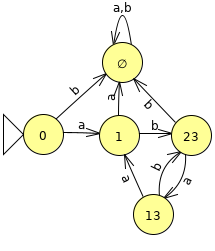
\includegraphics[scale=0.5]{TP05_8_d} \end{center}
\end{minipage}
\end{center}
\subsection{Exercise 9}
\begin{enumerate}
\item Accepts $a$, which is not a valid string per the exercise statement.
\item \label{itm:5_9_2} Enumerates all possible configurations for the blocks of size 3, thus complying with the statement.
\item Does not accept $acb$, although it complies with the exercise statement.
\item Accepts $aaa$, which is not a valid string per the exercise statement.
\end{enumerate}
The correct answer is \ref{itm:5_9_2}.
\pagebreak
\subsection{Exercise 10}
\begin{center} \begin{tabular}{r | c c}
	$\delta_D       $ & $0  $ & $1  $ \\ \hline
	$\rightarrow ^* q_1$ & $q_2$ & $q_3$\\
	$               q_2$ & $q_1$ & $q_3$\\
	$            ^* q_3$ & $q_2$ & $q_1$
\end{tabular} \end{center}
\subsubsection{Item a}
\begin{center} \begin{tabular}{r || c c | c c | c c}
	$k           $ & \multicolumn{2}{c |}{$0$} & \multicolumn{2}{c |}{$1$} & \multicolumn{2}{c}{$2$} \\ \hline
	$R_{11}^{(k)}$ & $\varepsilon$ & $\varepsilon$ & $\varepsilon+\varepsilon\varepsilon^*\varepsilon$& $\varepsilon$ & $\varepsilon+0(\varepsilon+00)^*0$ & $(00)^*$\\
	$R_{12}^{(k)}$ & $0$ & $0$ & $0+\varepsilon\varepsilon^* 0$ & $0$ & $0+0(\varepsilon+00)^*(\varepsilon+00)$ & $0(00)^*$\\
	$R_{13}^{(k)}$ & $1$ & $1$ & $1+\varepsilon\varepsilon^* 1$ & $1$ & $1+0(\varepsilon+00)^*(1+01)$ & $0^*1$\\
	$R_{21}^{(k)}$ & $0$ & $0$ & $0+0\varepsilon^*\varepsilon$ & $0$ & $0+(\varepsilon+00)(\varepsilon+00)^*0$ & $0(00)^*$\\
	$R_{22}^{(k)}$ & $\varepsilon$ & $\varepsilon$ & $\varepsilon+0\varepsilon^* 0$& $\varepsilon+00$ & $\varepsilon+00+(\varepsilon+00)(\varepsilon+00)^*(\varepsilon+00)$ & $(00)^*$\\
	$R_{23}^{(k)}$ & $1$ & $1$ & $1+0\varepsilon^* 1$ & $1+01$ & $1+01+(\varepsilon+00)(\varepsilon+00)^*(1+01)$ & $(00)^*(1+01)$\\
	$R_{31}^{(k)}$ & $1$ & $1$ & $1+1\varepsilon^*\varepsilon$ & $1$ & $1+(0+10)(\varepsilon+00)^*0$ & $(1+00)(00)^*$\\
	$R_{32}^{(k)}$ & $0$ & $0$ & $0+1\varepsilon^* 0$ & $0+10$ & $0+10+(0+10)(\varepsilon+00)^*(\varepsilon+00)$ & $(0+10)(00)^*$\\
	$R_{33}^{(k)}$ & $\varepsilon$ & $\varepsilon$ & $\varepsilon+1\varepsilon^* 1$& $\varepsilon+11$ & $\varepsilon+11+(0+10)(\varepsilon+00)^*(1+01)$ & $\varepsilon+(0+1)0^*1$
\end{tabular} \end{center}
\begin{alignat*}{2}
	R_{13}^{(3)}
	&= 0^*1+0^*1(\varepsilon +(0+1)0^*1)^*(\varepsilon +(0+1)0^*1)\\
	&= 0^*1+0^*1((0+1)0^*1)^*(\varepsilon +(0+1)0^*1)\\
	&= 0^*1((0+1)0^*1)^*(\varepsilon +(0+1)0^*1)\\
	&= 0^*1((0+1)0^*1)^*
\end{alignat*}
\begin{alignat*}{2}
	R_{11}^{(3)}
	&= (00)^* + 0^*1(\varepsilon+(0+1)0^*1)^* (1+00)(00)^* \\
	&= (00)^* + 0^*1((0+1)0^*1)^* (1+00)(00)^* 
\end{alignat*}
\begin{alignat*}{2}
	R_{11}^{(3)}+R_{13}^{(3)}
	&= 0^*1((0+1)0^*1)^* + (00)^* + 0^*1((0+1)0^*1)^* (1+00)(00)^* \\
	&= 0^*1((0+1)0^*1)^* + 0^*1((0+1)0^*1)^* (1+00)(00)^* + (00)^* \\
	&= 0^*1((0+1)0^*1)^*(\varepsilon + (1+00)(00)^*) + (00)^* \\
	&= 0^*1((0+1)0^*1)^*(\varepsilon + 1(00)^*+(00)^+) + (00)^* \\
	&= 0^*1((0+1)0^*1)^*(1(00)^*+(00)^*) + (00)^* \\
	&= 0^*1((0+1)0^*1)^*(\varepsilon + 1)(00)^* + (00)^* \\
	&= (00)^*  + 0^*1((0+1)0^*1)^*(\varepsilon + 1)(00)^*
\end{alignat*}
\subsubsection{Item b}
\begin{center}
\begin{minipage}{0.30\textwidth}
	\begin{center} 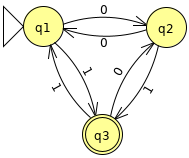
\includegraphics[scale=0.5]{TP05_10_b_1} \end{center}
	\begin{center} 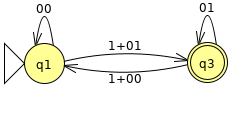
\includegraphics[scale=0.5]{TP05_10_b_2} \end{center}
\end{minipage}%
\begin{minipage}{0.60\textwidth}
	\begin{alignat*}{2}
	 	 & (00)^*(1+01)           &&(01 + (1+00)(00)^*(1+01))^*\\
		=& (00)^*(\varepsilon+0)1 &&(01 + 1(00)^*(1+01)+00(00)^*(1+01))^*\\
		=& 0^*1                   &&(01 + 1(00)^*(\varepsilon+0)1+00(00)^*(1+01))^*\\
		=& 0^*1                   &&(01 + 10^*1+00(00)^*(1+01))^*\\
		=& 0^*1                   &&(01 + 10^*1+00(00)^*(\varepsilon+0)1)^*\\
		=& 0^*1                   &&(01 + 10^*1+000^*1)^*\\
		=& 0^*1                   &&(01 +000^*1 + 10^*1)^*\\
		=& 0^*1                   &&(0(\varepsilon +00^*)1 + 10^*1)^*\\
		=& 0^*1                   &&(0(\varepsilon +0^+)1 + 10^*1)^*\\
		=& 0^*1                   &&(00^*1 + 10^*1)^*\\
		=& 0^*1                   &&((0+1)0^*1)^*
	\end{alignat*}
\end{minipage}
\end{center}
\begin{center}
\begin{minipage}{0.30\textwidth}
	\begin{center} 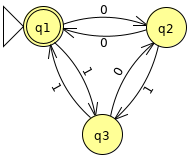
\includegraphics[scale=0.5,trim={0  7mm 0 0}]{TP05_10_b_1_2} \end{center}
	\begin{center} 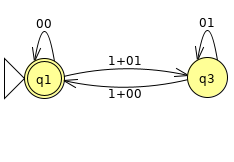
\includegraphics[scale=0.5,trim={0 20mm 0 0}]{TP05_10_b_2_2} \end{center}
	\begin{center} 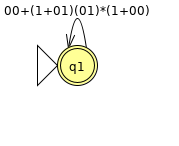
\includegraphics[scale=0.5,trim={0 20mm 0 0}]{TP05_10_b_3_2} \end{center}
\end{minipage}%
\begin{minipage}{0.60\textwidth}
	\begin{alignat*}{2}
	 	 & (00+(1+01)(01)^*(1+00))^*\\
		=& (00+(1+01)01^*(0+1))^* \\
		=& (00+(\varepsilon+0)101^*(0+1))^*
	\end{alignat*}
\end{minipage}
\end{center}
\begin{alignat*}{2}
	0^*1((0+1)0^*1)^* + (00+(\varepsilon+0)101^*(0+1))^*
\end{alignat*}
\subsection{Exercise 11}
The correct answer is NE.
\begin{center} 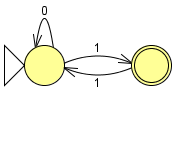
\includegraphics[scale=0.5]{TP05_11} \end{center}
}
